\documentclass[a4paper]{article}
\usepackage{pstricks}
\usepackage{amsmath}
\usepackage{graphicx}
\usepackage{pdfpages}
\usepackage{mathrsfs}

\setlength{\unitlength}{1.0mm}
\sloppy

\begin{document}

\title{Credit Stress Testing}
\author{Michal Mackanic (RMO)}
\date{April 2018}
\maketitle

\tableofcontents{}

\section{Stressing Migration Matrix}

\subsection{Introduction}
There seems to be consensus about migration matrix stressing as many
papers are based on Merton / Vasicek model and research by Peter Miu 
\& Bogie Ozdemir (see [1] for details). Only few papers follow different path, e.g. 
incorporating macroeconomic variables directly into estimation of 
probabilities of default.

\subsection{The Model}

Let us consider a firm that is clasified under rating group $i$. For the 
purpose of further analysis we assume that all firms within a 
rating group are homogenous, i.e. they are interchangeble in 
terms of default and migration probabilities.

We start with an assumption that firm's log asset value is normally distributed and can be expressed as
\begin{equation}
X_i = \sqrt{\rho} Z  + \sqrt{1 - \rho} \epsilon_i,
\end{equation}
where $Z \sim N[0, 1]$ represents the systematic and $\epsilon_i \sim 
N[0, 1]$ represents idiosyncratic risk factor, which are mutually independent. 
$\rho$ represents correlation between the asset returns and systematic 
risk factor $Z$. It follows that $Z$ is normally distributed with zero mean and standard deviation of one.

The above equation represents a cornerstone of 
well-known Merton model. Although rarely 
fulfilled in practice, the assumptions accepted in credit risk modelling.

Further, we assume that the firm defaults if its asset value falls 
below some threshold $TH_i$. Therefore, we can express probability of default as
\begin{multline}
PD_i = P[X_i < TH_i] = P[\sqrt{\rho}Z + \sqrt{1 - \rho} 
\epsilon_i < TH_i]=\\
P\left[\epsilon_i < \frac{TH_i - \sqrt{\rho}Z}{\sqrt{1 - 
\rho}}\right] = \Phi\left[\frac{TH_i - \sqrt{\rho}Z}{\sqrt{1 - 
\rho}}\right].
\end{multline}

A similar approach could be used for migration 
probabilities - probability that a counterparty migrates from rating 
$i$ to rating $j$ is
\begin{multline}
PM_{i,j} = P[TH_{i, j + 1} \le X_i < TH_{i, j}] =\\
P[TH_{i, j + 1} \le \sqrt{\rho}Z + \sqrt{1 - \rho} \epsilon_i < TH_{i, j}]=\\
\Phi\left[\frac{TH_{i, j} - \sqrt{\rho}Z}{\sqrt{1 - 
\rho}}\right] - \Phi\left[\frac{TH_{i, j + 1} - \sqrt{\rho}Z}{\sqrt{1 - 
\rho}}\right].
\end{multline}
Please note that the higher $j$, the worse the rating, i.e. $TH_{i, j} 
> TH_{i, j + 1}$.

To generalize, consider a migration matrix consisting of $N$ rating groups with 
the last rating group corresponding to default. Therefore we have to determine $N + 1$ thresholds for each rating 
group; boundary thresholds are $TH_{i, 1} = 
\infty$ and $TH_{i, N + 1} = -\infty$. Then
\begin{equation}
PM_{i,j} = \Phi\left[\frac{TH_{i, j} - \sqrt{\rho}Z}{\sqrt{1 - 
\rho}}\right] - \Phi\left[\frac{TH_{i, j + 1} - \sqrt{\rho}Z}{\sqrt{1 - 
\rho}}\right]
\end{equation}
for $j = 1, 2, ..., N$ with $PM_{i, N}$ being probability of default 
$PD_i$.

\begin{figure}[htp]
\centering
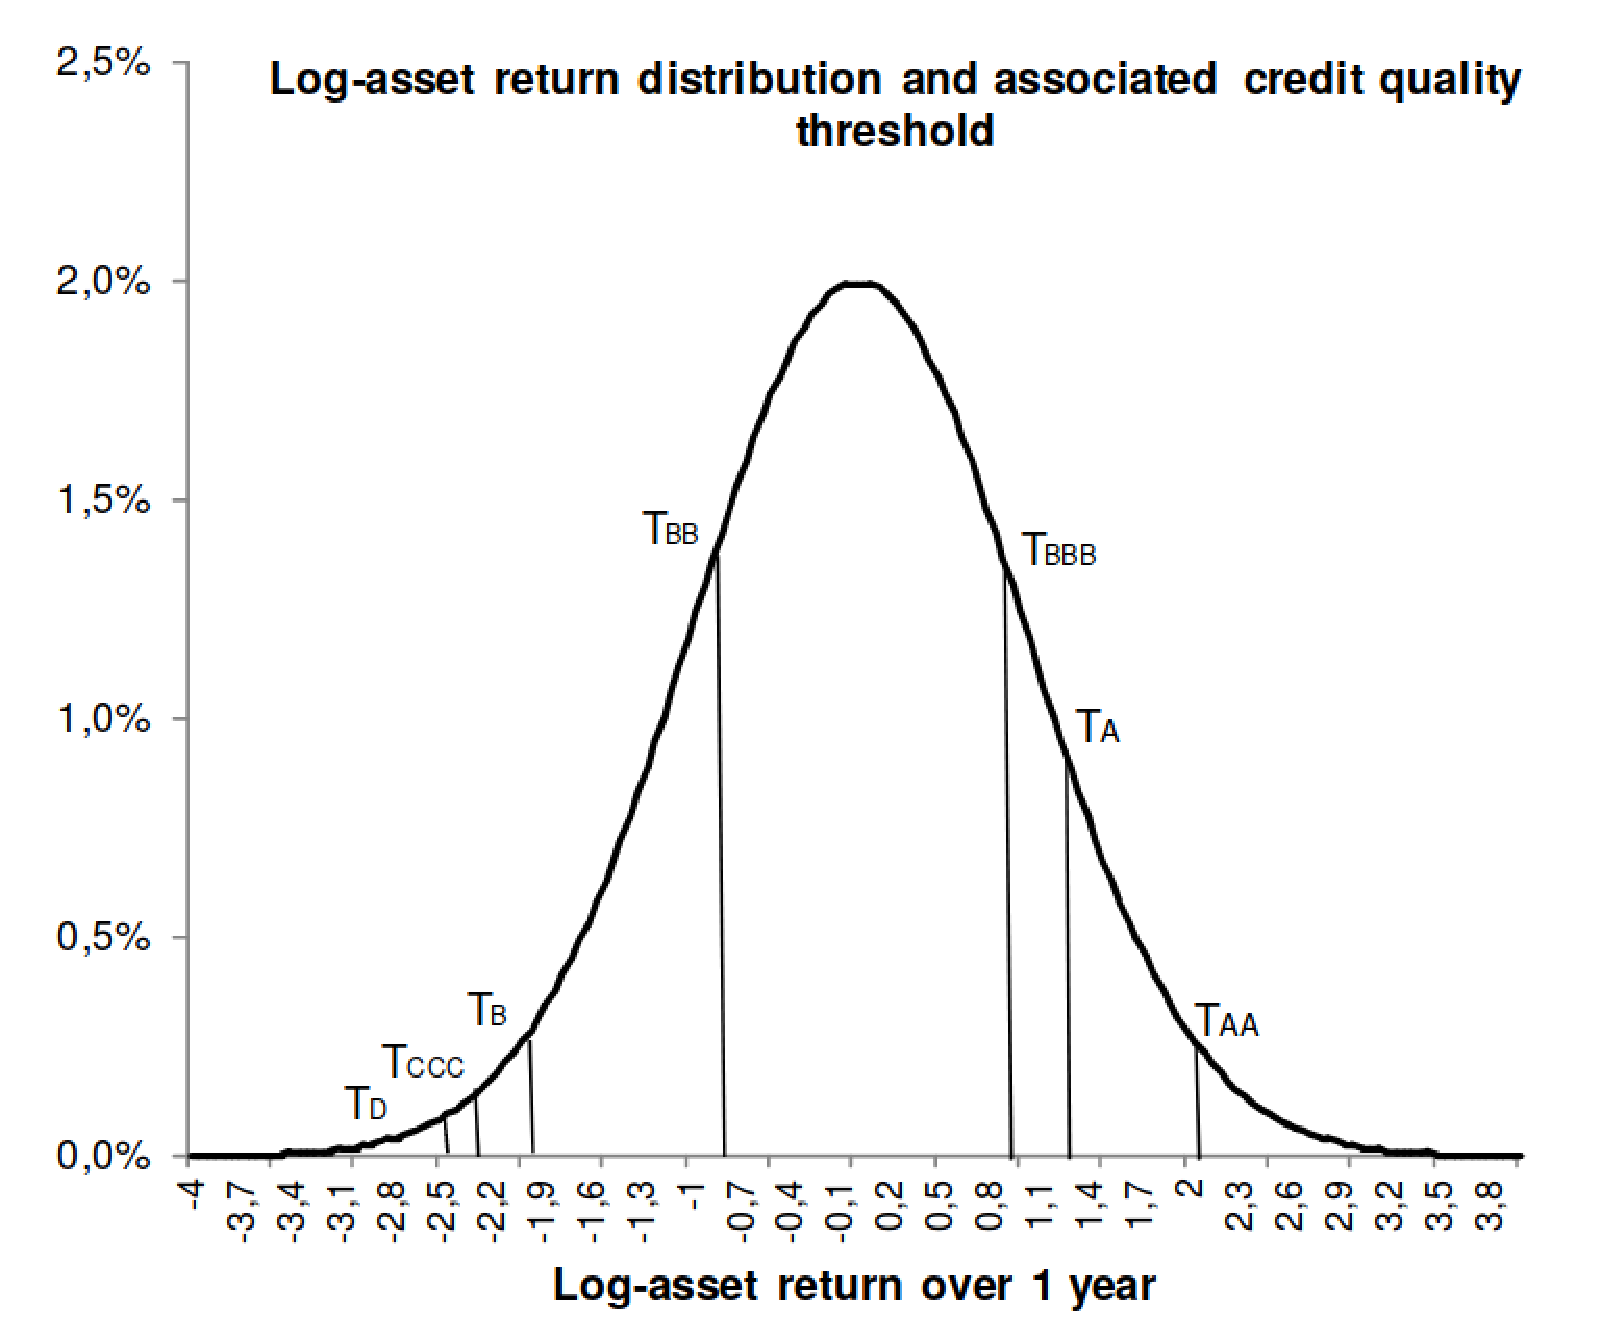
\includegraphics[scale = 0.35]{pictures/thresholds.eps}
\caption{Illustration of threshold concept; source [4]}
\label{thresholds}
\end{figure}


\subsection{Systematic Risk}

Remember that $Z$ in (2) represents systematic risk factor and hence 
we can think of $Z$ as being an economic cycle indicator. Therefore $Z$ is approximately 
zero during "average" time, greater than zero during economic boom and negative during recession.
Clearly, we can use $Z$ to determine probability of 
default conditioned on economic cycle.
\begin{equation}
PD_i = \Phi\left[\frac{TH_i - \sqrt{\rho}z}{\sqrt{1 - \rho}} | Z = 
z\right].
\end{equation}

We can use observed default rates as a proxy for probability of 
defaults. If we further realize that $TH_i = \Phi^{-1}[DR_i^{TTC}]$, where $DR_i^{TTC}$ is an average (aka through-the-cycle) default
rate observed for rating group $i$, equation (5) then turns into
\begin{equation}
DR_i^t= \Phi \left[\frac{\Phi^{-1}[DR_i^{TTC}] - \sqrt{\rho}z_t}{\sqrt{1 - \rho}} | Z = z_t \right].
\end{equation}
If we fix $\rho$ in line with Basel III methodology, we know all 
variables but $z_t$ in equation (6). Therefore, given historical default rates, we can 
determine $z_t$ as
\begin{equation}
z_t = \frac{\Phi^{-1}[DR_i^{TTC}] - \Phi^{-1}[DR_i^t]\sqrt{1 - \rho}}{\sqrt{\rho}}.
\end{equation}
Please note assumption $Z \sim N[0, 1]$ implies that $z_t$ should be at 
least approximately normally distributed with zero mean and variance of one.

In the next section systematic risk factor $Z$ will be linked to 
macroeconomic variables via a regression model. To get time series of 
$z_t$ that is sensitive to changes in macroeconomic variables, one 
should use default rates of low quality counterparties, e.g. non-investment 
grades. Since high credit quality counterparties are much less effected by 
economic cycles, one might observe few or even no defaults during 
economic downturn, which makes estimation of regression model 
rather problematic.\footnote{Please note that value $z_t$ of systematic risk factor 
$Z$ is for given time $t$ common to all rating groups. Therefore, at 
least in theory, it does not matter which rating group is used to 
determine $z_t$. However, it is rating groups with lower credit grade 
where the information is the most profound. It is even better to 
aggregate several lower rating groups to reduce noise in data.} See [1], footnote 19 for 
further comments.

\subsection{Macroeconomic Variables}

As explained above, given default rates $DR_i^t$ for time period $t$, average default rate $DR_i^{TTC}$ and
correlation $\rho$, we are able to determine values of systematic risk 
represented by $Z$ using equation (7). The next natural step is to find an appropriate 
regression model that links systematic risk factor to 
macroeconomic variables like GDP, unemployment, inflation, equity 
indices, credit spreads or interest rates. In other words, 
we are looking for a model in form of
\begin{equation}
z_t = \alpha + \sum_{m = 1}^M \beta_j Y_{m, t} + \varepsilon,
\end{equation}
where $Y_{m, t}$ represents a macroeconomic variable. 
Macroeconomic variables could be both current and lagged; it is also
advisable to include lagged $Z$ as an explanatory variable to account for persistence in observed default rates. An example 
of such a regression model is
\begin{equation}
z_t = \alpha + \beta_1 GDP_{t - 1} + \beta_2 IR^{5Y}_t + \beta_3 z_{t - 
1} + \varepsilon.
\end{equation}

Please note that explanatory variables should ideally follow standard normal 
distribution. Therefore one has to try various transformations 
(log-odd, log ratio or log transformation) and choose the one that fits 
normal distribution the best and normalize the transformed macro 
variable after that; see [2], page 8 for details.

Selection of appropriate explanatory variables is the most challenging 
part of the exercise because of numerous possible 
combinations (all potential macroeconomic variables both current and 
lagged \& their various transformations). Therefore one has to 
automate selection of appropriate explanatory variables, e.g. via LASSO 
regression. When selecting macroeconomic variables not only their statisticial significance, but also their importance
for scenario definition is to be considered.

\subsection{Threshold Calibration}

As stated above, we have fixed $\rho$ in line with Basel III methodology and 
determined values of $z_t$ using (7). That leaves us with thresholds 
to estimate. In the following text we will estimate thresholds using maximum likelihood method so 
that point-in-time migration matrices based on $z_t$ and the thresholds
matches observed migrations and defaults as closely as possible.

Consider rating group $i$. Let us assume that we have $T$ yearly observations 
of defaults and migrations within the rating group. We start with the lowest 
rating to estimate migration threshold $TH_{i, N}$.\footnote{Remember that $TH_{i, N + 1}$ equals to $-\infty$.} Default probabilities for $t = 
1, 2, ..., T$ equal
\begin{multline}
PD_i^t = PM_{i,N}^t = \Phi\left[\frac{TH_{i, N} - \sqrt{\rho}z_t}{\sqrt{1 - 
\rho}}\right] - \Phi\left[\frac{TH_{i, N + 1} - \sqrt{\rho}z_t}{\sqrt{1 - 
\rho}}\right] =\\
\Phi\left[\frac{TH_{i, N} - \sqrt{\rho}z_t}{\sqrt{1 - 
\rho}}\right] - \Phi\left[\frac{-\infty - \sqrt{\rho}z_t}{\sqrt{1 - 
\rho}}\right] = \Phi\left[\frac{TH_{i, N} - \sqrt{\rho}z_t}{\sqrt{1 - 
\rho}}\right].
\end{multline}
Please note that threshold $TH_{i, N}$ does not depend on time $t$. Let us 
assume we observed $k_{i,N}^t$ defaults out of $n_i^t$ counterparties 
within rating group $i$ during time period $t$. For a given threshold $TH_{i, N}$ 
probability of this event could be described via binomial distribution as
\begin{equation}
p_{i, N}^t = \binom{n_i^t}{k_{i, N}^t} \left(PM_{i,N}^t\right)^{k_{i, 
N}^t} \left(1 - PM_{i,N}^t\right)^{n_i^t - k_{i, N}^t}.
\end{equation}
Applying concept of maximum likelihood we have to maximize
\begin{equation}
LM_{i, N} = \sum_{t = 1}^T \log(p_{i, N}^t)
\end{equation}
through selection of appropriate threshold value $TH_{i, N}$. Optimal threshold value could be easily found through a grid seach method.

Once threshold $TH_{i, N}$ is estimated, we can continue with threshold 
$TH_{i, N - 1}$. Again, we estimate probability of observing $k_{i, N 
- 1}^t$ migrations within a portfolio of $n_i^t$ counterparties within time period $t$ as
\begin{equation}
PM_{i,N - 1}^t = \Phi\left[\frac{TH_{i, N - 1} - \sqrt{\rho}z_t}{\sqrt{1 - 
\rho}}\right] - \Phi\left[\frac{TH_{i, N} - \sqrt{\rho}z_t}{\sqrt{1 - 
\rho}}\right].
\end{equation}
Optimal value of threshold $TH_{i, N - 1}$ could be found using a grid 
search maximizing
\begin{equation}
LM_{i, N - 1} = \sum_{t = 1}^T \log(p_{i, N - 1}^t).
\end{equation}

The remaining thresholds could be found in the same manner.\footnote{The last threshold to estimate is $T_{i, 2}$ since $T_{i, 1}$ is set to $\infty$.} The
procedure is applied to all rating groups.

\subsection{Link Between Point-in-time and Through-the-cycle}

In the above text we implicitly estimated point-in-time migration 
matrices that fit the observed migrations and defaults. Once all thresholds are 
estimated, $z_t$ is plugged into (3) to construct the corresponding 
point-in-time migration matrix. Since through-the-cycle migration 
matrix corresponds to an "average" year, one can construct the 
matrix assuming $z_{TTC} = 0$ or $z_{TTC} = \frac{1}{T}\sum_{t = 1}^T 
z_t$.\footnote{Remember that $Z$ is supposed to 
be normally distributed with zero mean.} This also illustrates that historical window used 
for calibration should ideally consists of several full economic cycles.

\subsection{Stress Testing}

The following hierarchical steps summarize stress testing process of migration matrix.
\begin{enumerate}
\item Split historical data in several non-overlapping time periods $t = 1, 2, ..., T$. 
The periods typically represent quarters, half-years or years.
\item Determine number of observed migrations and defaults per rating group for each time period $t = 1, 2, ..., T$.
\item Using data from the previous step, determine aggregated default rates 
for non-investment rating groups for each time period $t = 1, 2, ..., T$.
\item Fix value of correlation $\rho$ in line with Basel III methodology.
\item Using default rates from step (3) determine values $z_t$ 
of systematic risk factor $Z$ for each time period $t = 1, 2, ..., T$.
\item Construct an appropriate regression model that establishes a 
link between systematic risk factor $Z$ and macroeconomic variables.
\item Using observed defaults and migrations during time periods $t = 1, 2, ..., T$ calibrate thresholds, which define historical point-in-time 
migration matrices and consistent through-the-cycle migration matrix (which could be for example determined via $z_{TTC} = 0$).
\item Take stressed macroeconomic variables and determine corresponding 
value $z_{stress}$ of systematic risk factor $Z$ using regression model 
introduced in step (6).
\item Using $z_{stress}$ and thresholds calibrated in step (7) 
construct point-in-time migration matrix that corresponds to stressed 
macroeconomic variables.
\end{enumerate}

\section{Stressing LGD}

\subsection{Introduction}

Unlike in case of stressed migration matrix, it seems that consensus is
still not reached for stressed LGD. There are several papers 
on the topic which differ greatly in their approach to the problem. 
Paper [3] seems to give the most pragmatic approach.

\subsection{The Model}

Although existence of positive correlation between probability of default and LGD is 
generally accepted, there is only little empirical research on the 
topic. Paper [3] offers an interesting approach to the problem. The 
main idea is that distributions of LGD and probability of default are comonotonic. 
This means that LGD quantiles map directly to quantiles of probability of default, 
e.g. 20\% LGD quantitle corresponds 20\% quantile probability of default 
quantile. In other words, if we are able to determine quantile for 
stressed probability of default, we can use the quantile to determine 
corresponding stressed LGD.

The paper assumes that through-the-cycle probability of default is known. Using Vasicek model, quantile 
of a certain stressed probability of default is
\begin{equation}
q = \Phi \left[\frac{\sqrt{1 - \rho} \Phi^{-1}[PD_{stress}] - 
\Phi^{-1}[PD_{TTC}]}{\sqrt{\rho}}\right].
\end{equation}

It further supposes that stressed loss rate also obeys Vasicek distribution. 
Using the above determined quantile $q$ and expected loss $EL$ we can calculate the 
corresponding stressed loss rate as
\begin{multline}
loss_{stress} = \Phi \left[\frac{\Phi^{-1}[EL] + 
\sqrt{\rho}\Phi^{-1}[q]}{\sqrt{1 - \rho}} \right] = \\
\Phi\left[\Phi^{-1}[PD_{stress}] - \frac{\Phi^{-1}[PD_{TTC}] - 
\Phi^{-1}[EL]}{\sqrt{1 - \rho}}\right].
\end{multline}

Stressed LGD could be then  easily determined as
\begin{equation}
LGD_{stress} = \frac{loss_{stress}}{PD_{stress}} = \frac{\Phi\left[\Phi^{-1}[PD_{stress}] - 
k\right]}{PD_{stress}}
\end{equation}
where
\begin{equation}
k = \frac{\Phi^{-1}[PD_{TTC}] - \Phi^{-1}[EL]}{\sqrt{1 - \rho}}
\end{equation}
is called LGD risk index and which fully determines LGD function. Figure (\ref{lgd-function}) illustrates LGD function for several levels of $k$.

\begin{figure}[htp]
\centering
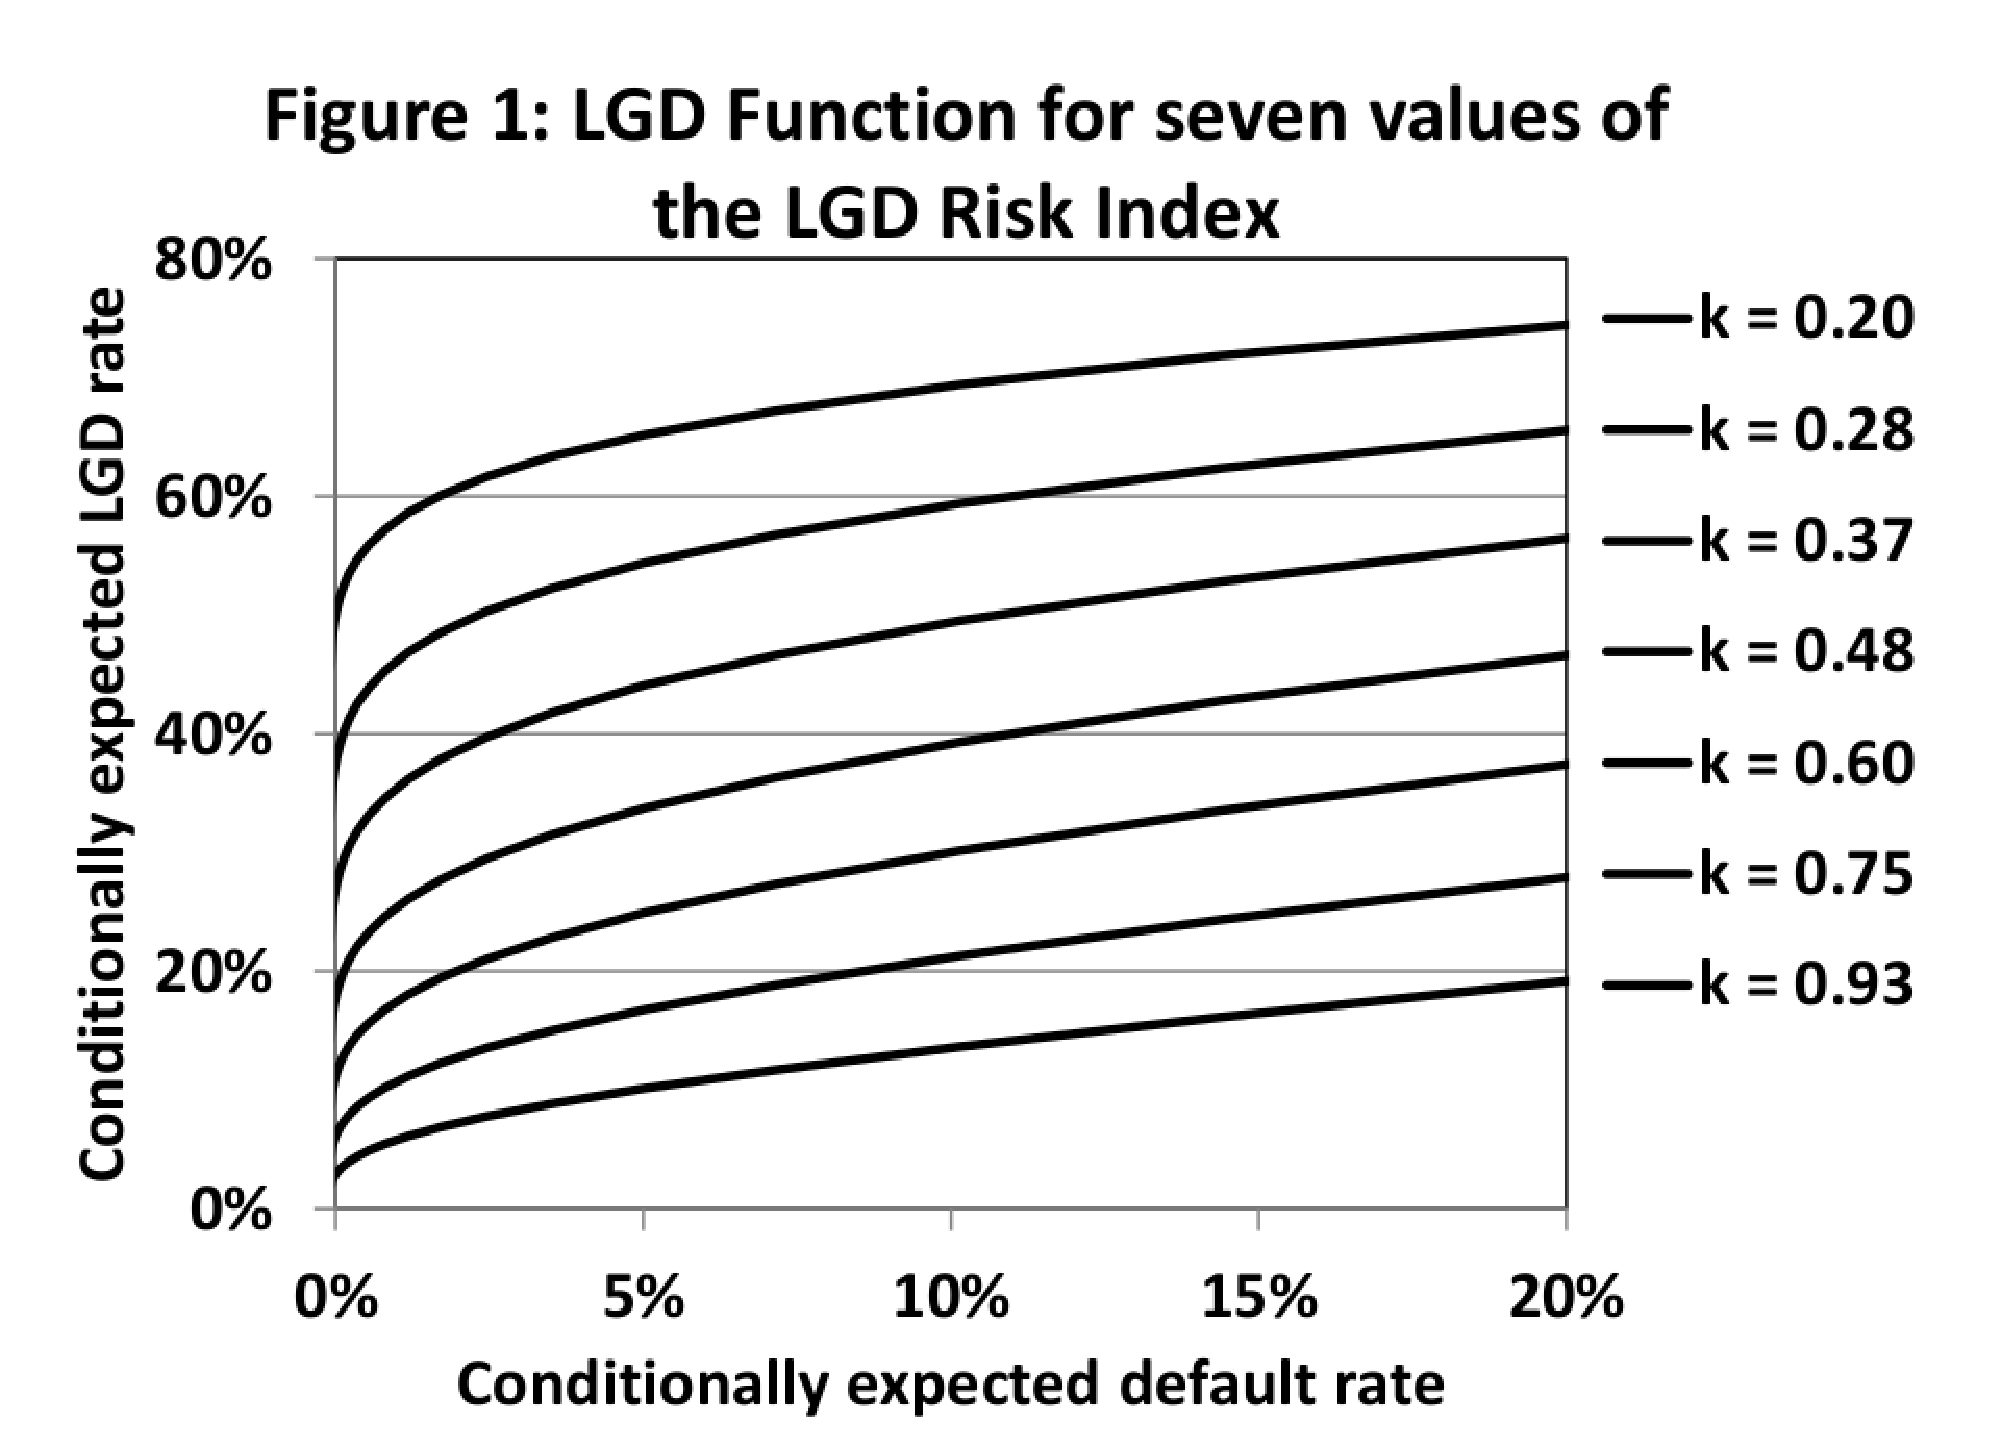
\includegraphics[scale = 0.35]{pictures/lgd-function.eps}
\caption{LGD function for different levels of $k$; source [3]}
\label{lgd-function}
\end{figure}

Clearly, the above methodology of LGD stressing stands on assumption that stressed loss rate follows Vasicek distribution.
Also, somewhat surprisingly, one only needs through-the-cycle probability of default,
expected loss and correlation to fully determine stressed LGD.\footnote{Please note that
correlation $\rho$ used in LGD model is the same as that used to stress probability of default model.}
Due to limited number of parameters LGD function can change only its level but not its shape; this is apparent from figure (\ref{lgd-function}).
Paper does not provide any economic explanation of the assumption. Appropriateness of Vasicek distribution is underpinned by analysis of US corporate bond market;
it is not not clear whether the approach could extended to, for example, retail portfolios. On the other hand, proposed LGD function is simple to calibrate and fits into concept
of probability of default.

\begin{center}
\begin{figure}[htp]
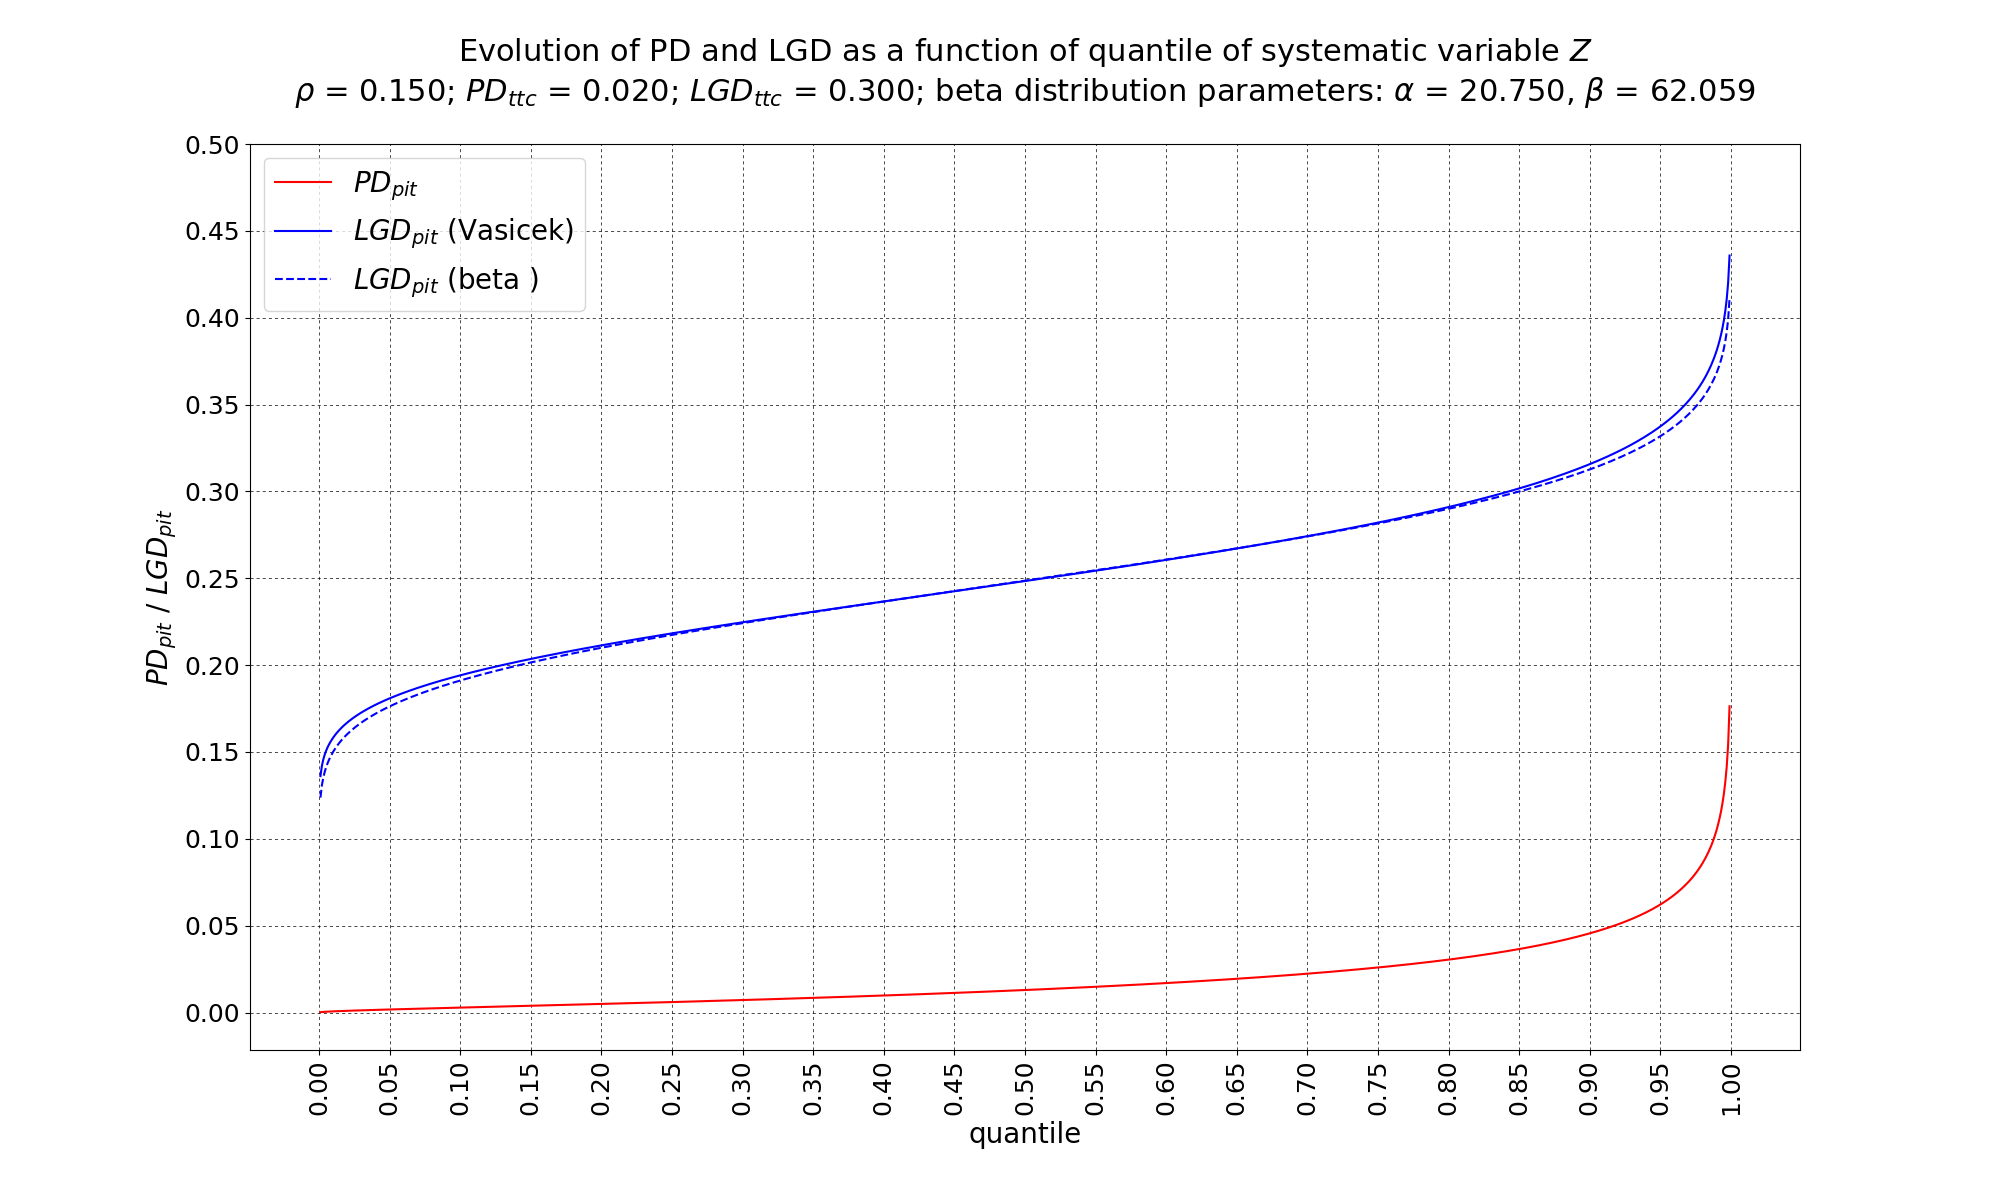
\includegraphics[scale = 0.45, angle = 270]{pictures/lgd-test.eps}
\caption{LGD function based on Vasicek and beta distribution}
\label{lgd-test}
\end{figure}
\end{center}

However, using comonotonicity, the main idea of [3], the method could be easily extended to other probability distributions.
After all, alternative distributions are used in [3] to justify
LGD function based on Vasicek distribution. One of possible candidates is beta distribution, which could be (a) calibrated on LGD
observed through out economic cycle or (b) based on expert opinion. Similar to original approach, we use quantile implied by stressed
probability of default to determine stressed LGD. For example, if stressed probability
of default implies 20\% quantile of systematic risk factor $Z$, we associate it with LGD that corresponds to 20\% quantile of the
beta distribution. Using beta distribution we can mimic LGD function of (17) as
illustrated in figure (\ref{lgd-test}) (correlation of 15\%, through-the-cycle probability of default of 2.00\% and through-the-cycle
LGD of 30\%, which implies expected loss of 6.00\%; corresponding beta function is based
expert opinion predicting 21\% LGD for 20\% quantile and 29\% LGD for 80\% quantile).

\subsection{Alternative for Mortgage Portfolio}

An appealing alternative for mortgage portfolio is introduced in [5]. The idea behind the paper is rather intuitive - since real estate collateralizes
mortgage loan financing its purchase, we can argue that LGD is driven by loan-to-value of mortgage portfolio and real estate price shocks. Disadvantage of the approach
is that LGD is determined by secured recoveries only, i.e. collateral realization, and that other possibly important macroeconomic drivers are ignored.

To illustrate the main idea, consider a mortgage loan with
current loan-to-value of 60\% and recovery rate of 80\%. Translated into numbers, a fictive loan of 600 EUR is covered by a real estate with current value of 1,000 EUR,
which would yield 800 EUR if sold. In other words, financial institution does not suffer a loss in case of default.
However, consider 30\% shock to real estate prices. Assuming that the shock reduces recovery rate to 56\%\footnote{The updated recovery rate was derived as $0.80 \cdot (1 - 0.30) = 0.56$ or 56\%.}, sale of the real estate would yield only 560 EUR.
Therefore, in case of default financial institution would suffer a loss of 40 EUR. This implies LGD of 6.67\%.

\begin{center}
\begin{figure}[htp]
\centering
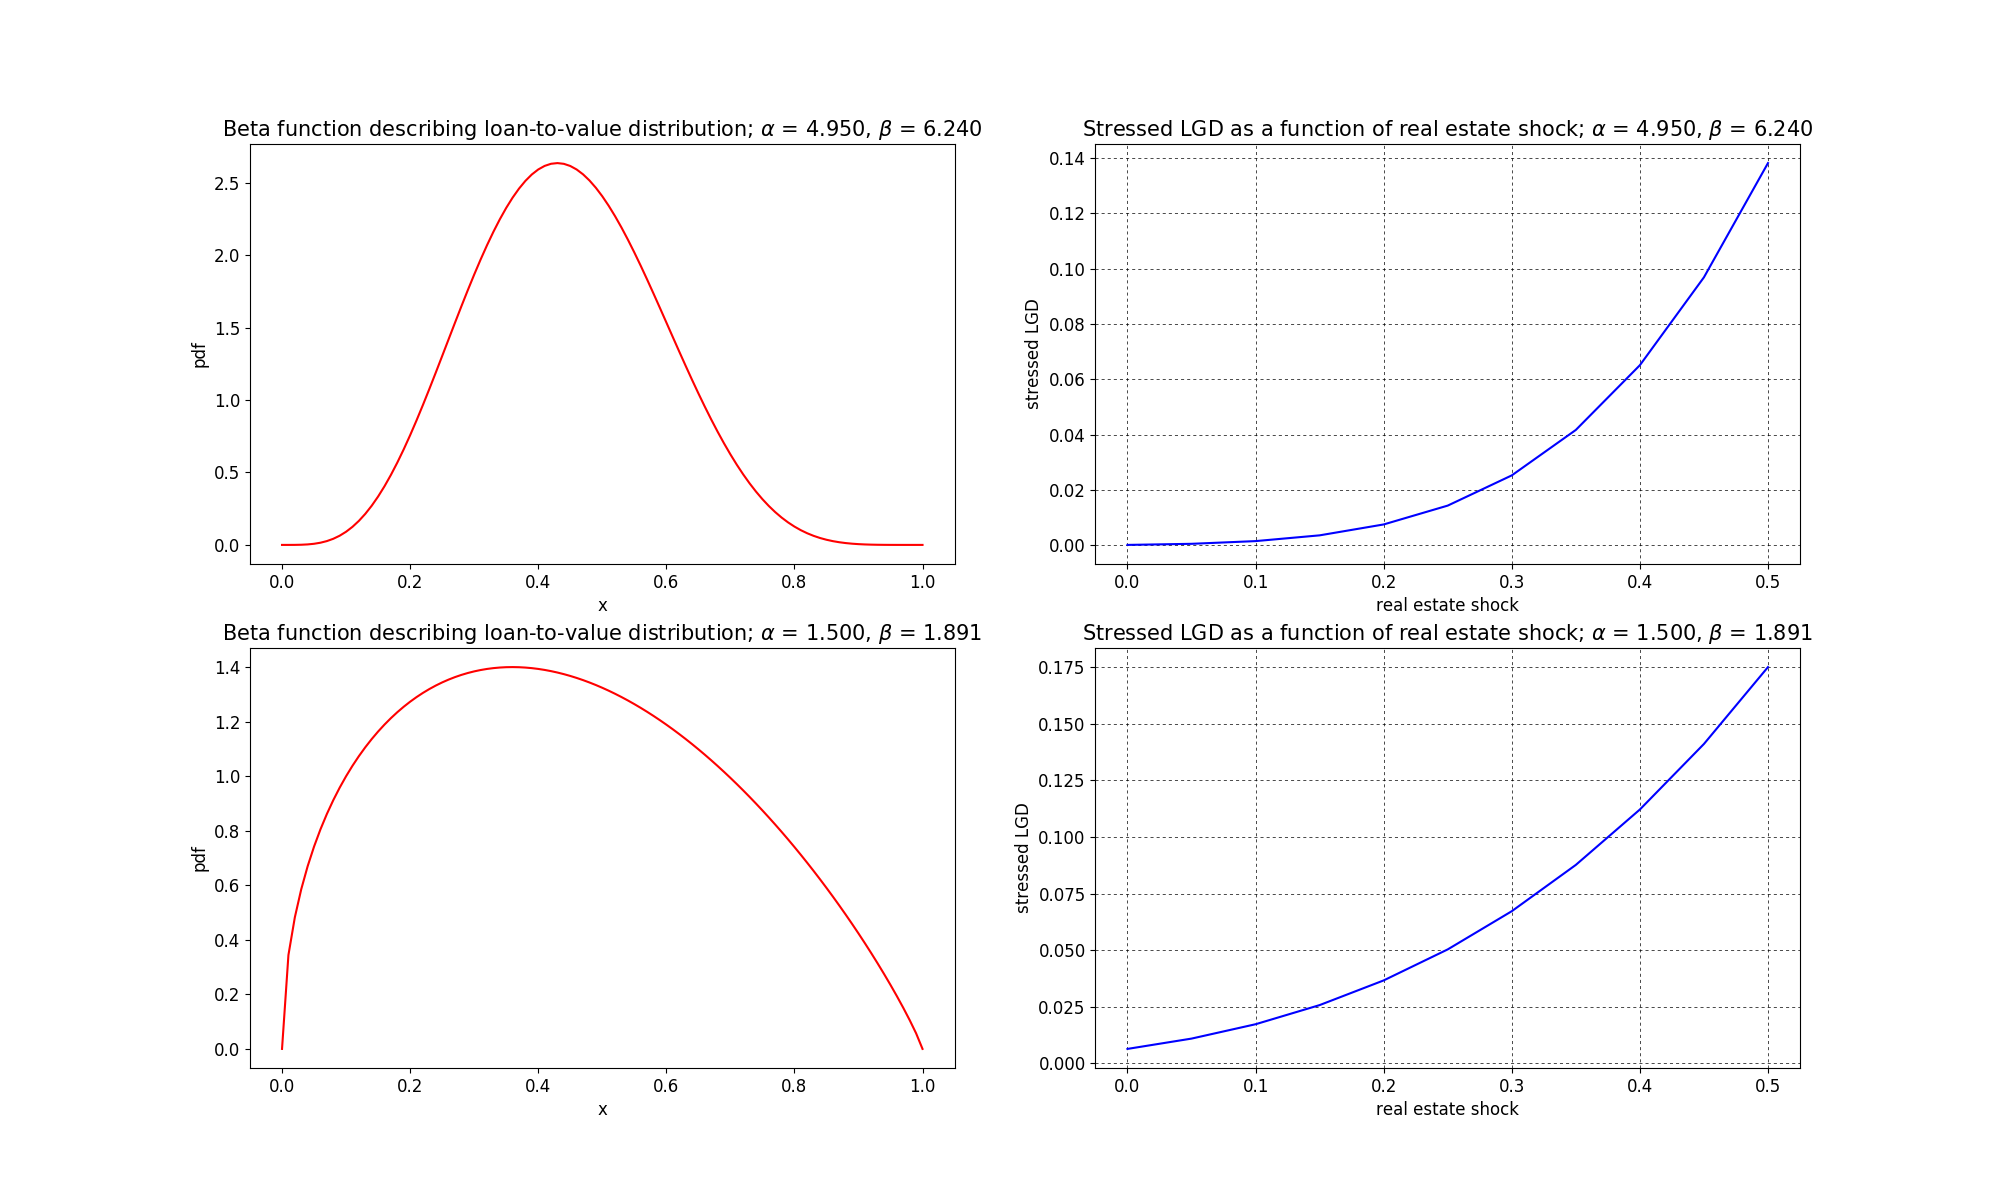
\includegraphics[scale = 0.45, angle = 270]{pictures/lgd-mortgages.eps}
\caption{Loan-to-value based LGD as a function of real estate price shock}
\label{lgd-mortgages}
\end{figure}
\end{center}

Although relatively straight-forward, the approach cannot be used in practice because of large number of mortgages - treating mortgages on individual basis is not computationally feasible.
However, the paper offers an analytical formula that is based on assumption that portfolio's
loan-to-value could be described through a variable $X$ following beta distribution with probability function of
\begin{equation}
	f(x) = \frac{x^{\alpha - 1}(1 - x)^{\beta - 1}}{B(\alpha, \beta)}
\end{equation}
for $x \in [0, 1]$, where $B(\alpha, \beta) = \frac{\Gamma(\alpha)\Gamma(\beta)}{\Gamma(\alpha + \beta)}$ is beta function. LGD conditioned by a particular loan-to-value could be modelled
for some deterministic recovery rate $rr \in [0, 1]$ as\footnote{The formula could be derived as $LGD = \max\left[0, \frac{LTV - RR}{LTV}\right] = \max\left[0, 1 - \frac{RR}{LTV}\right] = 1 - \frac{RR}{\max[RR, LTV]}$.}
\begin{equation}
	Y := g(X) = 1 - \frac{rr}{\max[rr, X]}.
\end{equation}
Bringing (19) and (20) together, we get
\begin{multline}
	E[Y] = \int_0^1 g(x)f(x)dx = 1 - F_{X}(rr) - rr \frac{\alpha + \beta - 1}{\alpha - 1}(1 - F_{X'}(rr)),
\end{multline}
where $F_{X'}(a)$ is cumulative distribution of random variable $X'$ following beta distribution with parameters $\alpha - 1$ and $\beta$.{}
In this way we expressed the mean portfolio LGD as a function
of the mean recovery rate and of the two parameters $\alpha$ and $\beta$ that capture the portfolio's loan-to-value distribution. LGD is stressed through stressing average recovery rate.

An important point made in the paper is that portfolios with wider loan-to-value distribution have higher LGD.
This is illustrated by figure (\ref{lgd-mortgages}) for two fictive mortgage portfolios with the same expected loan-to-value of 44\%.\footnote{Expected value of a random variable $X$ following beta distribution is defined as $E[X] = \frac{\alpha}{\alpha + \beta}$.}
For a real estate shock of -30\%, we expect average LGD to be under 3\% for the first but around 7\% for the second fictive portfolio.

\section{References}

\noindent [1] Stress-Testing Probability of Default and Migration Rate with Respect to Basel II Requirements - Peter Miu, Bogie Ozdemir; October 2008
\vskip 0.2in
\noindent [2] Validation Report on PD stress test modelling guidelines and application to Belgian portfolios - Chris De Langhe (WRB-WVA); January 2015
\vskip 0.2in
\noindent [3] Loss given default as a function of the default rate - Jon Frye; September 2013
\vskip 0.2in
\noindent [4] Stress-testing bank's corporate credit portfolio - Olivier de Bandt, Nicolas Dumontaux, Vincent Martin, Denys Medee; March 2013
\vskip 0.2in
\noindent [5] Stress Testing the Credit Risk of Mortgage Loans: The Relationship between Portfolio-LGD and the Loan-to-Value Distribution - Christian Greve, Lutz Hahnenstein; August 2014

\end{document}
